\documentclass[draft,11pt]{article}

%packages
\usepackage[british]{babel}
\usepackage{mathtools}              % AMS Math Package
\usepackage{amsthm}                 % Theorem Formatting
\usepackage{physics}
\usepackage{graphicx}               % Allows for eps images
% \usepackage{multicol}             % Allows for multiple columns
% \usepackage{sectsty}                % custom sectionals
\usepackage{titlesec}
\usepackage[small]{caption}         % small captions
\usepackage{newtxtext,newtxmath}    % font change
% \usepackage{lmodern}
\usepackage[T1]{fontenc}
\usepackage[utf8]{inputenc}
\usepackage{csquotes}
\usepackage{enumerate}              % custom enumerations
\usepackage{url}                    % nice url fonts
\usepackage[a4paper,top=2.54cm,bottom=2.54cm,left=3.18cm,right=3.18cm]{geometry}
\usepackage[separate-uncertainty=true]{siunitx}
\usepackage{float}
\usepackage[style=ieee,backend=biber]{biblatex}
\usepackage{tikz}
\usepackage{parskip}
\usepackage{booktabs}
\usepackage{multirow}
%end packages

\usepackage{subcaption}

%commands
\renewcommand{\labelenumi}{(\alph{enumi})}
\newtheorem{prop}{Proposition}
\newtheorem{thm}{Theorem}[section]
\newtheorem{lem}[thm]{Lemma}
\theoremstyle{definition}
\newtheorem{dfn}{Definition}
\theoremstyle{remark}
\newtheorem*{rmk}{Remark}

\bibliography{report}

\titlelabel{\thetitle.\quad}

\titleformat*{\section}{\normalfont\bfseries}
\titlespacing*{\section}{0pt}{1.1\parskip}{.33\parskip}
\titleformat*{\subsection}{\normalfont\bfseries}
\titlespacing*{\subsection}{0pt}{1.1\parskip}{.33\parskip}
\titleformat*{\subsubsection}{\normalfont\bfseries}
\titlespacing*{\subsubsection}{0pt}{1.1\parskip}{.33\parskip}

\let\oldvec=\vec
\renewcommand{\vec}[1]{\vb{#1}}
\newcommand{\uvec}[1]{\vu{#1}}

\DeclareSIUnit\solarmass{M_{\odot}}

%cover page command
\newcommand{\makecover}[5]{
\thispagestyle{empty}
\setcounter{page}{0}
\begin{center}\LARGE{\bf #1}\vskip 24pt \normalsize{#2}\hspace*{\fill}\\
#3\vskip 12pt School of Physics and Astronomy\\The University of Manchester\vskip 12pt Theory Computing Project Report\vskip 12pt #4\end{center}\vskip 54pt

\section*{Abstract}
#5
\newpage}
%end of coverpage command

\pagestyle{plain}%page numbers in footer

\begin{document}
    \makecover
    {Neutron stars}
    {Tomoi Goto and Luis Caceres Cueva}
    {10139083 and 9916879}
    {May 2019}
    {In this project, the effects of the internal structure of the neutron stars on their radius and mass were examined by solving the Tolman-Oppenheimer-Volkoff equation with appropriate equation of states using 4th order Runge-Kutta method. For the equation of state, pure Fermi gas consisting of proton and neutron was used, and different strength of nuclear interactions were considered by varying the nuclear incompressibility $K_0$. For $K_{0}$ values of \SI{100}{\mega\electronvolt}, \SI{175}{\mega\electronvolt}, \SI{250}{\mega\electronvolt}, \SI{325}{\mega\electronvolt}, and \SI{400}{\mega\electronvolt} the maximum masses were determined to be \SI{1.36}{\solarmass}, \SI{2.01}{\solarmass}, \SI{2.30}{\solarmass}, \SI{2.27}{\solarmass}, and \SI{1.97}{\solarmass}, respectively. The resulting mass-radius relations were compared with the actual observation of low mass X-ray binaries and neutron star merger, and the EOS with a $K_0$ of \SI{175}{\mega\electronvolt} and \SI{250}{\mega\electronvolt} was the most consistent with the observations.}
    
    \section{Introduction}
        Neutron stars, stellar remnants created after supernovae of $>\SI{5}{\solarmass}$ stars, have a mean density of around \SI{e18}{\kilogram\per\meter\cubed} and are in the low temperature regime of nuclear matter \parencite{shapiro.teukolsky.1983/bh.wd.ns.co}. Compared to high temperature but low density enviroments in particle accelerators such as LHC in CERN, this highly dense but low temperature state of matter is very difficult to recreate in laboratories on Earth \parencite{graber.andersson.2017/ns.lab}. Therefore, the study of neutron stars offers an opportunity for studying nuclear matter at extremely high density, conditions which are not fully studied yet.  
        
        To further illustrate, there are multiple models for the equation of state of the matter, with different composition (e.g. strange quark, hyperions, etc.) or different interactions, which result in different mass-radius curves for neutron stars \cite{graber.andersson.2017/ns.lab}. Hence, by comparing a calculated mass-radius relation with the actual observation of the radii and masses of neutron stars, one could find better constraints of the parameters in order to find better mathematical models of these high density states.
        
        In this report, we study the Fermi gas model with pure neutron asymmetric nuclear interaction, and calculate the mass-radius relation at different strengths of the nuclear interaction, parametrised by the nuclear compressibility at saturation $K_{0}$. We compare our results with other proposed equation of states from the scientific literature as well as with the actual observed masses and radii acquired from low mass X-ray binaries and the neutron star merger event of GW170817.
    
    \section{Theory}
        \subsection{Structure equation}
            For a fluid in hydrostatic equilibrium, we have \[\rho\vec{f}=\grad{p},\] where $\rho$ is the density, $\vec{f}$ is the force per unit mass and $p$ is the pressure. Hence, when the force is Newtonian gravity, \[\dv{p}{r}=-\frac{G\rho M}{r^{2}},\] where $r$ is the distance from the centre of the neutron star, $p=p(r)$ is the pressure at radius $r$, $\rho=\rho(r)$ is the density at radius $r$, $M=M(r)$ is the mass of the inner shell of radius $r$ and $G$ is the gravitational constant. In a general relativistic treatment, some correction factors must be incorporated \parencite{silbar.reddy.2004/neutron.stars}, and hence we write the Tolman-Oppenheimer-Volkoff equation (Equation \ref{eq/tov.pressure}),
            \begin{align}
                \label{eq/tov.pressure}\dv{p}{r}&=-\frac{G\rho M}{r^{2}}\qty[1+\frac{p}{\epsilon}]\qty[1+\frac{4\pi r^{3}p}{Mc^{2}}]\qty[1-\frac{2GM}{c^{2}r}]^{-1}\\
                \label{eq/tov.mass}\dv{M}{r}&=4\pi r^{2}\rho,
            \end{align}
            where $\epsilon=\epsilon(r)$ is the energy density at radius $r$ and $c$ is the speed of light. Equation \ref{eq/tov.mass} is straightforward from the definition of the mass of an inner spherical shell.

            
        \subsection{Fermi gas model} % TODO cite pdf and koonin
            The neutron matter inside of a neutron star can be modeled as a degenerate Fermi gas at temperature $T=\SI{0}{\kelvin}$.\footnote{This is a valid approximation because the Fermi temperature at the densities we are considering (up to \SI{e21}{\kilogram\per\meter\cubed}) is in the order of \SI{e12}{\kelvin}, which is much higher than core temperatures of very massive stars at the end of their lives ($\sim\SI{e9}{\kelvin}$).} In this model, the energy density can be written as \parencite{koonin.1986/computational.physics/rk4.white.dwarf}
            \[\epsilon=2\int_{0}^{k_{F}}E(k)g(k)\dd{k},\] where $g(k)=k^{2}/2\pi^{2}$ is the density of states function, $E(k)=\sqrt{\hbar^{2}c^{2}k^{2}+m^{2}c^{4}}$ is the relativistic energy of the state with wavenumber $k$, and $m$ is the mass of the fermion (in this case, a neutron). With the substitution $y=\hbar k/mc$ and defining a function \parencite{koonin.1986/computational.physics/rk4.white.dwarf} \[I(x)\equiv \frac{3}{8x^{3}}\qty[x(1+2x^{2})(1+x^{2})^{1/2}-\log(x+\sqrt{1+x^{2}})]\] in terms of dimensionless $x=\hbar k_{F}/mc$ to simplify the notation, the energy density can be written as \[\epsilon=\epsilon_{0}x^{3}I(x),\] where $\epsilon_{0}=m^{4}c^{5}/\pi^{2}\hbar^{3}$ is a constant.
            
            Calculating the number density is simpler, \[n=2\int_{0}^{k_{F}}g(k)\dd{k}=\frac{k_{F}^{3}}{3\pi^{2}}=n_{0}x^{3},\] where $n_{0}=m^{3}c^{3}/3\pi^{2}\hbar^{3}$ is a constant. Hence, calculating the mass density is straightforward, \[\rho=mn_{0}x^{3}=\rho_{0}x^{3},\] where $\rho_{0}=mn_{0}$ is another constant.
            
            In summary, we have the following quantities in terms of dimensionless $x$ (which in turn is a function of the Fermi wavenumber $k_{F}$):
                \begin{align}
                    x&=\frac{\hbar k_{F}}{mc}\\
                    n&=n_{0}x^{3},\\
                    \label{eq/fermi/mass.density}\rho&=\rho_{0}x^{3},\\
                    \label{eq/fermi/energy.density}\epsilon&=\epsilon_{0}x^{3}I(x).
                \end{align}
                
            Hence, we can calculate the pressure \begin{equation}\label{eq/fermi/pressure}p=\qty(\pdv{U}{V})_{N}=n^{2}\qty[\pdv{n}(\frac{\epsilon}{n})]_{N}=\frac{1}{3}\epsilon_{0}x^{4}I'(x).\end{equation}

        
        \subsection{Fermi gas with nucleon interactions}
            Extending the Fermi gas model, we can write that the energy per nucleon for symmetric matter (i.e. number of protons equal to the number of neutrons) is given by \parencite{silbar.reddy.2004/neutron.stars} \[\frac{\epsilon(n)}{n}=mc^{2}I(x)+V(u)\] where $x=\sqrt[3]{n/n_{0}}$ is as in the previous section, $V(u)$ is the nucleon interaction potential written in terms of the dimensionless quantity $u=n/n_{1}$, where $m$ is the mass of a nucleon (i.e. we ignore the small difference between the proton and neutron mass) and $n_{1}$ is the saturation density (i.e. the density at which the potential $V$ is the minimum and is equal to the binding energy per nucleon of elemental matter). We also make the assumption that this potential applies to all neutron stars. % TODO explain this
            
            For small $x$, we can approximate $I(x)$ as \[I(x)\approx1+\frac{3}{10}x^{2}.\] Writing $x^{3}=\eta u$, where $\eta=n_{1}/n_{0}$ is the ratio between constants, we have \begin{equation}\label{eq/symmetric.energy}\frac{\epsilon(n)}{n}=mc^{2}\qty(1+\frac{3\eta^{2/3}}{10}u^{2/3})+V(u).\end{equation} % TODO explainl why we can use non relativistic approximation
            
            We can parametrise the equations for antisymmetric matter using a parameter $\alpha$ such that $n_{p}=(1-\alpha)n/2$ and $n_{n}=(1+\alpha)n/2$ where $n_{p}$ and $n_{n}$ are the proton density and neutron density, respectively \parencite{silbar.reddy.2004/neutron.stars}. Hence, we can write an approximation for the energy per nucleon of antisymmetric matter \parencite{prakash.ainsworth.lattimer.1988/eos}, \begin{equation}\label{eq/antisymmetric.energy}E(n,\alpha)=E(n,0)+\alpha^{2}S(n)\end{equation} where $E(n,0)$ is the energy per nucleon of symmetric matter given by Equation \ref{eq/symmetric.energy} and $S(n)$ is the symmetry breaking energy. Following Prakash et al. \cite{prakash.ainsworth.lattimer.1988/eos}, we use \begin{equation}\label{eq/symmetry.breaking}S(n)=E_{N}(2^{2/3}-1)\qty(u^{2/3}-F(u))+S_{0}F(u)\end{equation} where $u=n/n_{1}$ as before, $S_{0}=\SI{30}{\mega\electronvolt}$ \parencite{prakash.lattimer.2001/ns.structure.eos} is the bulk symmetry energy parameter, $F(u)$ is an arbitrary function such that $F(0)=0$ and $F(1)=1$ and \[E_{N}=\frac{3}{10}mc^{2}\eta^{2/3}\] is the kinetic energy per nucleon at equilibrium density $n=n_{1}$. Thus we can write the energy per nucleon for pure neutron matter ($\alpha=1$) as \[E(n,1)=\frac{\epsilon}{n}=mc^{2}+E_{N}u^{2/3}+V(u)+E_{N}(2^{2/3}-1)\qty(u^{2/3}-F(u))+S_{0}F(u).\] Now we can find an expression for the pressure, \[p=n^{2}\pdv{n}\qty(\frac{\epsilon}{n})=E_{N}n_{1}u^{2}\qty[\frac{2}{3}u^{-1/3}+\frac{V'(u)}{E_{N}}+(2^{2/3}-1)\qty(\frac{2}{3}u^{-1/3}-F'(u))+\frac{S_{0}}{E_{N}}F'(u)].\] To simplify calculations we define \[J(u)\equiv u^{2}\qty[\frac{2}{3}u^{-1/3}+\frac{V'(u)}{E_{N}}+(2^{2/3}-1)\qty(\frac{2}{3}u^{-1/3}-F'(u))+\frac{S_{0}}{E_{N}}F'(u)]\] such that we can write \[p=E_{N}n_{1}J(u).\]
            
            \subsubsection{The symmetric nucleon potential}\label{sec/symmetric.potential}
                So far, we have an expression for the equation of state as the pressure in terms of a function $J(u)$ of density $u=n/n1$, but this function in turn is written in terms of the nucleon interaction potential $V(u)$, for which we do not yet have an expression.
                
                In this work, we use the potential proposed by Bludman and Dover \cite{bludman.dover.1980/extrapolation.skyrme.eos}. This form of the nucleon interaction potential is based on the empirical Skyrme interaction for nuclear matter and is modified to account for higher densities than atomic nuclear densities while ensuring that the sound speed in such matter is below the speed of light \cite{bludman.dover.1980/extrapolation.skyrme.eos}. This potential can be written as \parencite{silbar.reddy.2004/neutron.stars} \begin{equation}\label{eq/symmetric.potential}V(u)=\frac{A}{2}u+\frac{Bu^{\sigma}}{(1+\sigma)(1+C_{1}u^{\sigma-1})},\end{equation} where $A$, $B$, $C_{1}$ and $\sigma$ are constants chosen to fit the parameters of nuclear matter at saturation nuclear densities \parencite{bludman.dover.1980/extrapolation.skyrme.eos}.
                
                Hence, using Equation \ref{eq/symmetric.energy} to express the energy per nucleon, we must have:
                \begin{enumerate}
                    \item the energy per nucleon has a minimum at the saturation density $n=n_{1}$, \begin{equation}\label{eq/symmetric.energy/saturation.minimum}\qty(\dv{u}\qty[\frac{\epsilon(n)}{n}])_{u=1}=0;\end{equation}
                    \item the value of the energy per nucleon at the minimum must be equal to the binding energy per nucleon $E_{B}=-\SI{16}{\mega\electronvolt}$ \parencite{silbar.reddy.2004/neutron.stars}, \begin{equation}\label{eq/symmetric.energy/binding.energy}\frac{\epsilon(n_{1})}{n_{1}}-mc^{2}=E_{B};\end{equation}
                    \item the value of the compressibility at the saturation density must be $K_{0}$ which has a value between \SI{100}{\mega\electronvolt} and \SI{400}{\mega\electronvolt} \parencite{silbar.reddy.2004/neutron.stars,prakash.ainsworth.lattimer.1988/eos},\footnote{In this work, we will fit the parameters of the nucleon interaction potential for different values of $K_{0}$.} \begin{equation}\label{eq/symmetric.energy/compressibility}K(n_{1})=9\dv{p}{n}=K_{0};\end{equation}
                    \item the value of $C_{1}$ is chosen such that the speed of sound in the matter is lower than the speed of light \parencite{bludman.dover.1980/extrapolation.skyrme.eos}, \begin{equation}\label{eq/symmetric.energy/speed.of.sound}\qty(\frac{c_{s}}{c})^{2}=\pdv{p}{\epsilon}<1.\end{equation}
                \end{enumerate}

                The potential, although empirical, can be interpreted physically. Given that $A$ is negative, the linear term represents the attractive strong force interaction of nearest neighbour nucleons. The other term instead represents the multiple body repulsive interactions with neighbours \parencite{bludman.dover.1980/extrapolation.skyrme.eos} (such as Coulombic or degeneracy pressure interactions).
            
        \subsection{Simultaneous measurement of masses and radii of neutron stars}
            There are number of methods for measuring the mass of a neutron star, but the measurements of low-mass X-ray binaries are particularly useful, since not only the mass but also the radius can be determined simultaneously \parencite{ozel.paulo.2016/masses.radii.eos}. There are two methods for determining the radius of the neutron star in the LMXB, one is to measure the thermal emmision from a quiescent LMXB, and the other is to measure the flux produced by the thermonuclear bursts \parencite{ozel.paulo.2016/masses.radii.eos}.
            
            Low mass X-ray binaries have a donor star ($M<\SI{1.5}{\solarmass}$) that transfers materials which then accretes on the neutron star \parencite{tauris.2003/xray.binary}. When the LMXB is in a quiescent period, the spectrum of the neutron star's thermal radiation can be analyzed to obtain the angular size of the neutron star, from which the radius can be determined \parencite{ozel.psaltis.2016/radius.oberve}.
            
            LMXB can also undergo thermonuclear bursts, which are caused by the ignition of helium on the surface of the neutron star \parencite{ozel.paulo.2016/masses.radii.eos}. This results in the expansion of neutron star's photosphere due to the radiation pressure, which then reaches equilibrium and Eddington luminosity. As the burst cools down the photosphere shrinks, and by measuring the flux when the photosphere touches the neutron star, the radius of the neutron star can be calculated using the expression for the Eddington luminosity \parencite{ozel.psaltis.2016/radius.oberve}.
            
            Other than the observations of LMXB in the electromagnetic spectrum, the advent of gravitational wave detectors made it possible to measure the total mass of a system of 2 neutron stars and their radii by observing merging events. In particular, the  radii and masses of the neutron stars in the event GW170817 has been calculated by the LIGO Scientific Collaboration and Virgo Collaboration \cite{ligo.virgo.2019/prop.of.ns.merger.GW170817,ligo.virgo.2018/GW170817.ns.radii}. In this report we use the radius inferred from the effect of the tidal deformation of the neutron stars on the signal of the gravitational wave, as presented in the paper by LIGO \cite{ligo.virgo.2018/GW170817.ns.radii}.
    
    \section{Methodology}
        \subsection{Runge-Kutta integration and mass-radius relation}
            We used 4th order Runge-Kutta method to integrate the structure equation for the values of density and mass as a function of radius. To perform the integration for a given EOS, initial density was set, and then the integration was terminated when the density reached 0, where at that point the final radius and the mass were recorded. By repeating this procedure for a range of different initial densites, the mass-radius relation was obtained for a given EOS.
            
            The main source of error in the Runge-Kutta method is the truncation error, which can be estimated by performing integration on two different step sizes $h_{1}=2h$ and $h_{2}=h$, and using the results $Y_{1}$ and $Y_{2}$ in the formula  \parencite{lotkin.1951/rk.accuracy} \[E_{2}=(Y_{1}-Y_{2})/15\] where $E_{2}$ is the estimated error when the step size is $h_{2}$. In our case we performed first integration at a given step size, and then performed another integration with twice the step size to then calculate the error on mass $M_{\text{err}}$ when the density reaches 0. After trying several step size with different EOS and intial densities, we found that for the step size of $h=\SI{1}{\meter}$ the error on the mass $M_{\text{err}}$ stays in the range between \SI{e-10}{\solarmass} to \SI{e-5}{\solarmass}, much smaller than the calculated masses of the neutron stars which are around \SI{1}{\solarmass}, so this step size was chosen for calculating all the EOS.
            
        \subsection{Singularities in the integration}
            Given that the RK4 integration is started at the centre of the neutron star, it is necessary to deal with the terms in the TOV equation of the form $M/r$ or $r/M$, which are indeterminate as $r\to0$. To resolve this, we start at a very small $r=\varepsilon\sim\SI{1}{\milli\meter}$, with an inner mass $M=\frac{4}{3}\pi\rho_{c}\varepsilon^{3}$ where $\rho_{c}$ is the density at the centre of the neutron star. Effectively, we consider that at the centre of the neutron star there is a very small sphere with uniform density $\rho_{c}$. This resolves the singularity.
            
        \subsection{Choice of free parameters and functions in the nucleon interaction EOS}
            As described in Section \ref{sec/symmetric.potential}, the parameters of the symmetric potential (Equation \ref{eq/symmetric.potential}) are $A$, $B$, $\sigma$ and $C_{1}$ which are fitted to the properties of nuclear matter at saturation density (Equations \ref{eq/symmetric.energy/saturation.minimum}, \ref{eq/symmetric.energy/binding.energy} and \ref{eq/symmetric.energy/compressibility}). The other constraint is an inequality (Equation \ref{eq/symmetric.energy/speed.of.sound}) and hence we have some freedom in choosing one of the parameters. Specifically, we set $C_{1}=0.3$, as Prakash \emph{et al.} \parencite{prakash.ainsworth.lattimer.1988/eos} did. Similarly, in the symmetry breaking energy (Equation \ref{eq/symmetry.breaking}) we choose $F(u)=\sqrt{u}$ which is one of the forms considered by Prakash \emph{et al.} as it reproduces the energy symmetry of more realistic calculations \parencite{prakash.ainsworth.lattimer.1988/eos}.
            
            Given that the compressibility at saturation density $K_{0}$ is not well determined \parencite{silbar.reddy.2004/neutron.stars}, we performed calculations for five different values of $K_{0}$ between \SI{100}{\mega\electronvolt} and \SI{400}{\mega\electronvolt}.
    
    \section{Results and discussion}
        \subsection{Comparison between Fermi gas model and nucleon interaction model}
            As shown in Figure \ref{fig/comparison.our.models}, there is a clear difference between the Fermi gas models with Newtonian structure and the GR structure. Given that the GR correction terms shown in Equation \ref{eq/tov.pressure} are all positive and greater than one, they effectively ``amplify'' the effect of gravity \parencite{silbar.reddy.2004/neutron.stars} and hence for a given initial mass density, the resulting neutron star will be smaller and less massive, as shown in the figure.
            
            \begin{figure}[h]\begin{center}
                \begin{subfigure}[b]{.49\textwidth}
                    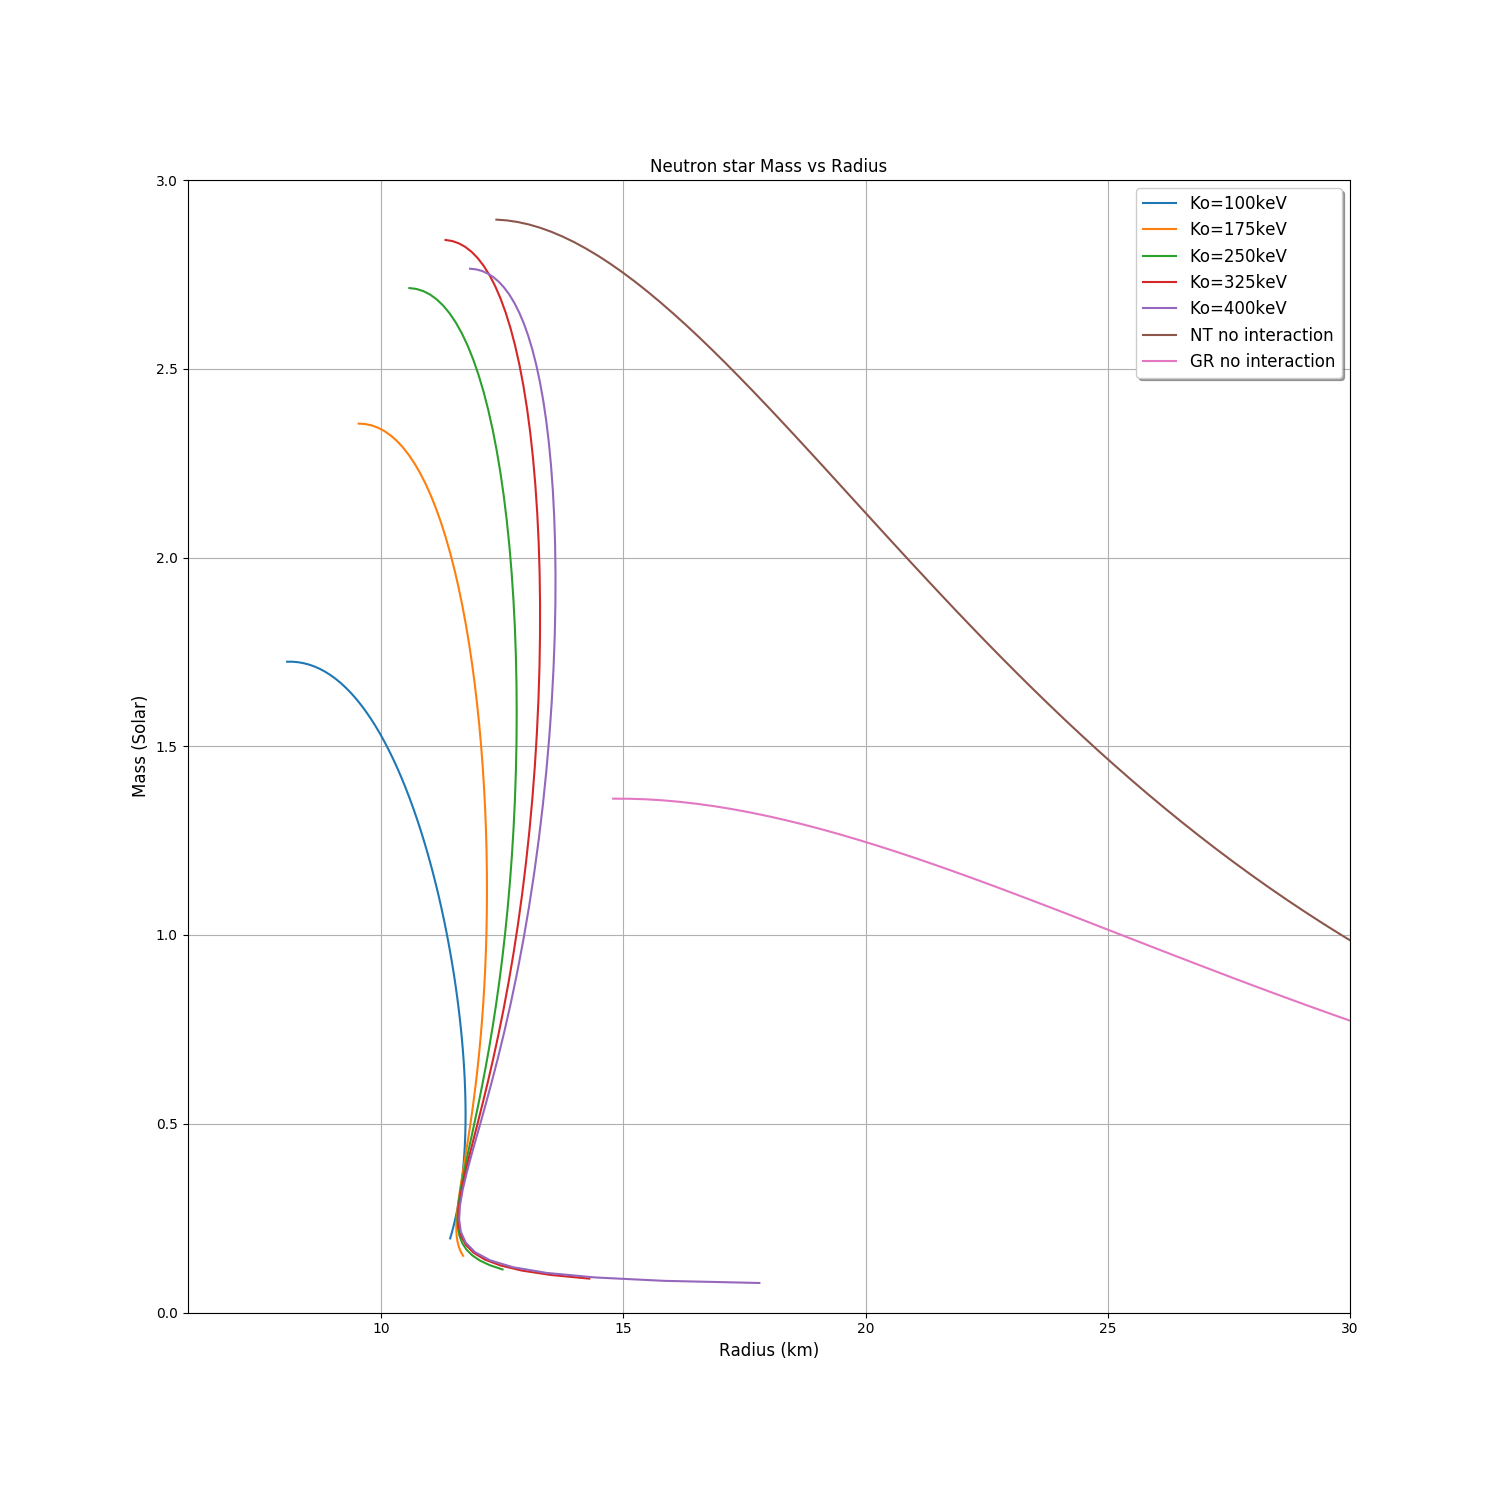
\includegraphics[width=\textwidth]{eos_compare_our_model}
                    \caption{Comparison between Fermi gas model and model with nucleon interactions}\label{fig/comparison.our.models}
                \end{subfigure}
                \begin{subfigure}[b]{.49\textwidth}
                    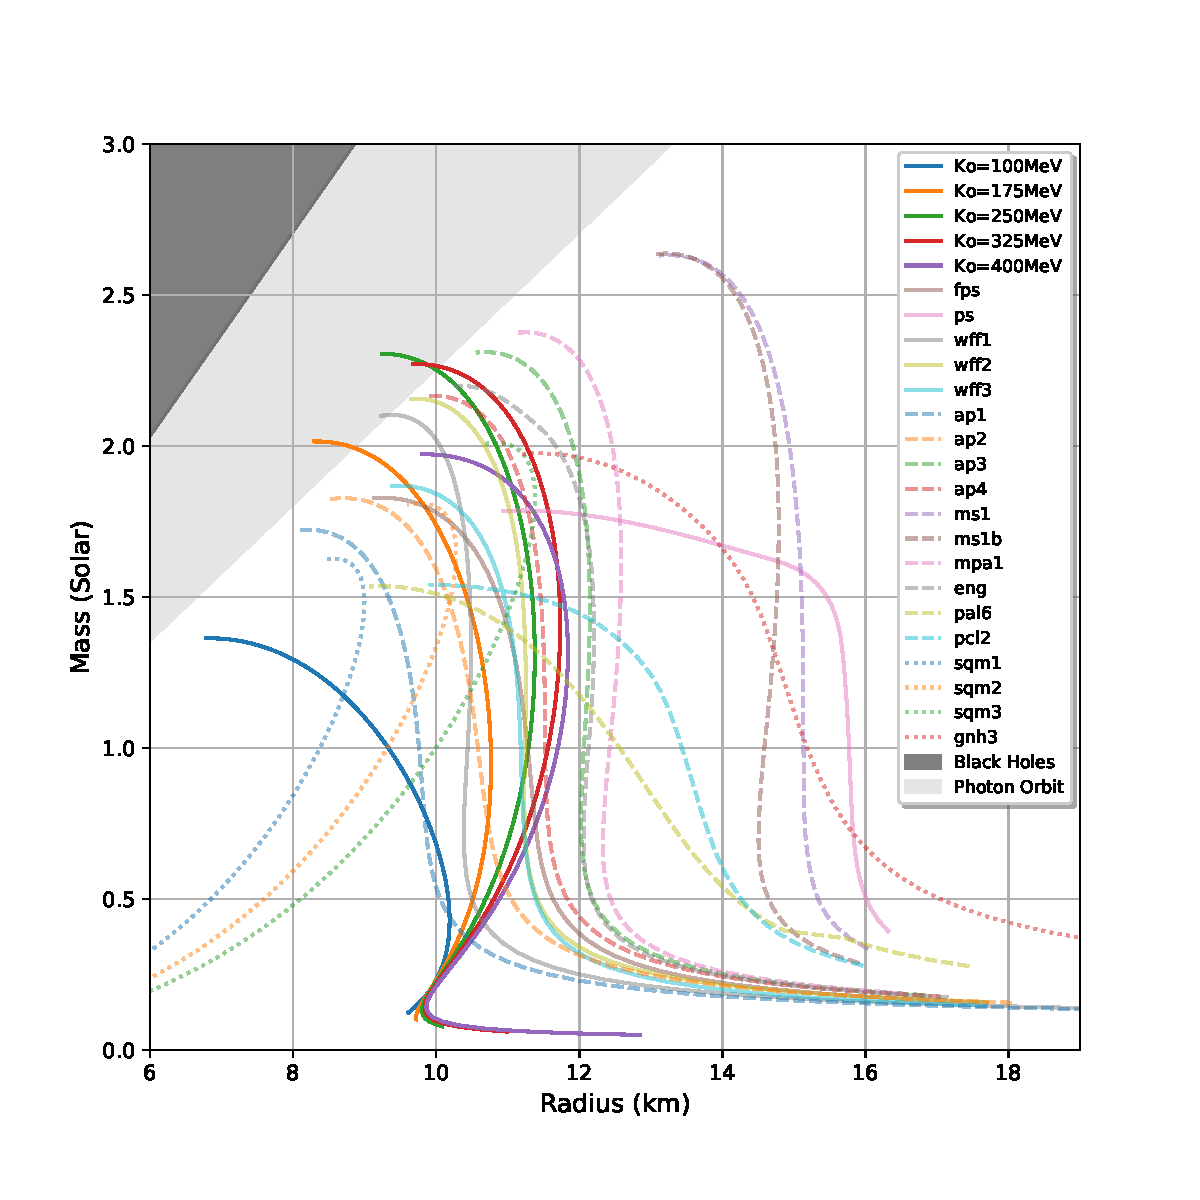
\includegraphics[width=\textwidth]{eos_compare_paper}
                    \caption{Comparison between our models and other models from the literature}\label{fig/comparison.paper}
                \end{subfigure}
                \caption{Comparison between different equation of state models}
            \end{center}\end{figure}
            
            Additionally, the simpler Fermi gas model produces less compact neutron stars compared to the model that accounts for nucleon interactions. This is as expected because the Fermi gas model only considers a repulsive interaction due to degeneracy pressure, while the other model includes the attractive strong interaction between neutrons.
            
            \begin{table}[h]\begin{center}
                \caption{Maximum masses and radii at maximum mass of neutron stars for a given nuclear incompressibility $K_0$}\label{tab/max.mass}
                \begin{tabular}{ccc}
                    \toprule
                    $K_{0}$ (\si{\mega\electronvolt}) & $M_{\text{max}}$ (\si{\solarmass}) & $R_{\text{max}}$ (\si{\kilo\meter}) \\
                    \midrule
                    \num{100} & \num{1.36} & \num{6.78}\\
                    \num{175} & \num{2.01} & \num{8.30}\\
                    \num{250} & \num{2.30} & \num{9.25}\\
                    \num{325} & \num{2.27} & \num{9.68}\\
                    \num{400} & \num{1.97} & \num{9.80}\\
                    \bottomrule
                \end{tabular}
            \end{center}\end{table}
            
            The calculated maximum mass of the neutron stars for the nucleon interaction EOS are listed in the Table \ref{tab/max.mass}.
        
        \subsection{Comparison with other EOS models from the literature}
            By comparing with the other EOS in Figure \ref{fig/comparison.paper}, we see that our EOS lies close to the EOS that consists of neutron and proton, such as wff \parencite{wff.1988} and ap \parencite{ap.1998}. The EOSs that deviate from the shape of our EOS assume that additional matters are present in the neutron star other than the protons and the neutrons, such as strange quark matters for sqm \parencite{sqm.pcl.1995}, pions for ps \parencite{ps.1975}, quarks and hyperons for pcl \parencite{sqm.pcl.1995}, and so on. 

        
        \subsection{Comparison with actual neutron star measurement data}
            \begin{figure}[h]\begin{center}
                \begin{subfigure}[b]{.49\textwidth}
                    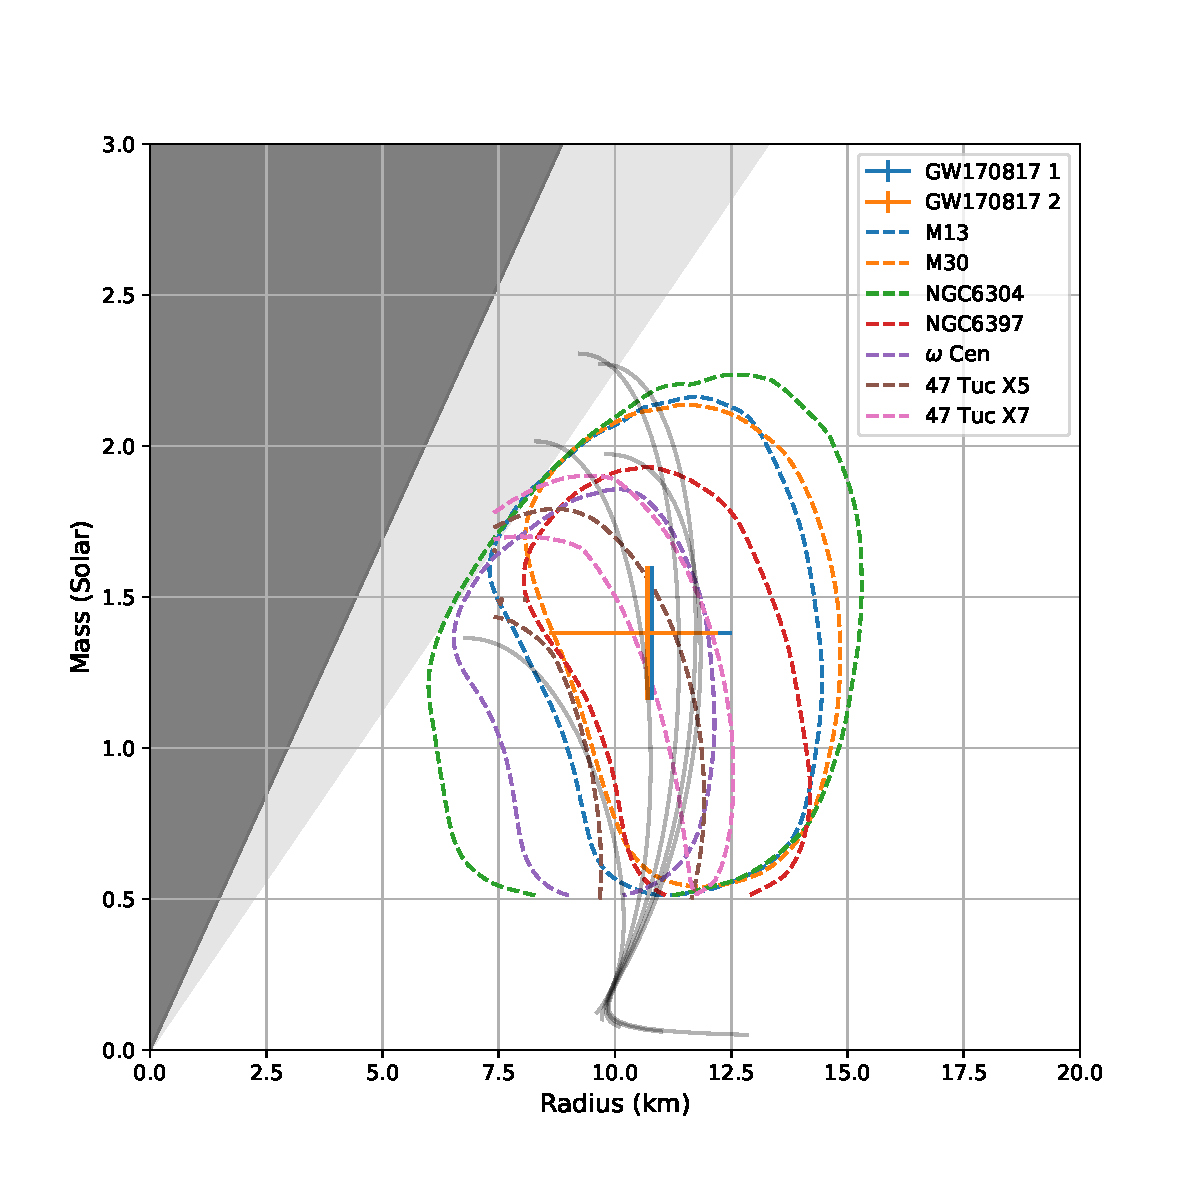
\includegraphics[width=\textwidth]{eos_compare_obsv1_GW}
                    \caption{Comparison between our model and the data from the quiescent LMXBs and GW event}\label{fig/quiescent.LMXB}
                \end{subfigure}
                \begin{subfigure}[b]{.49\textwidth}
                    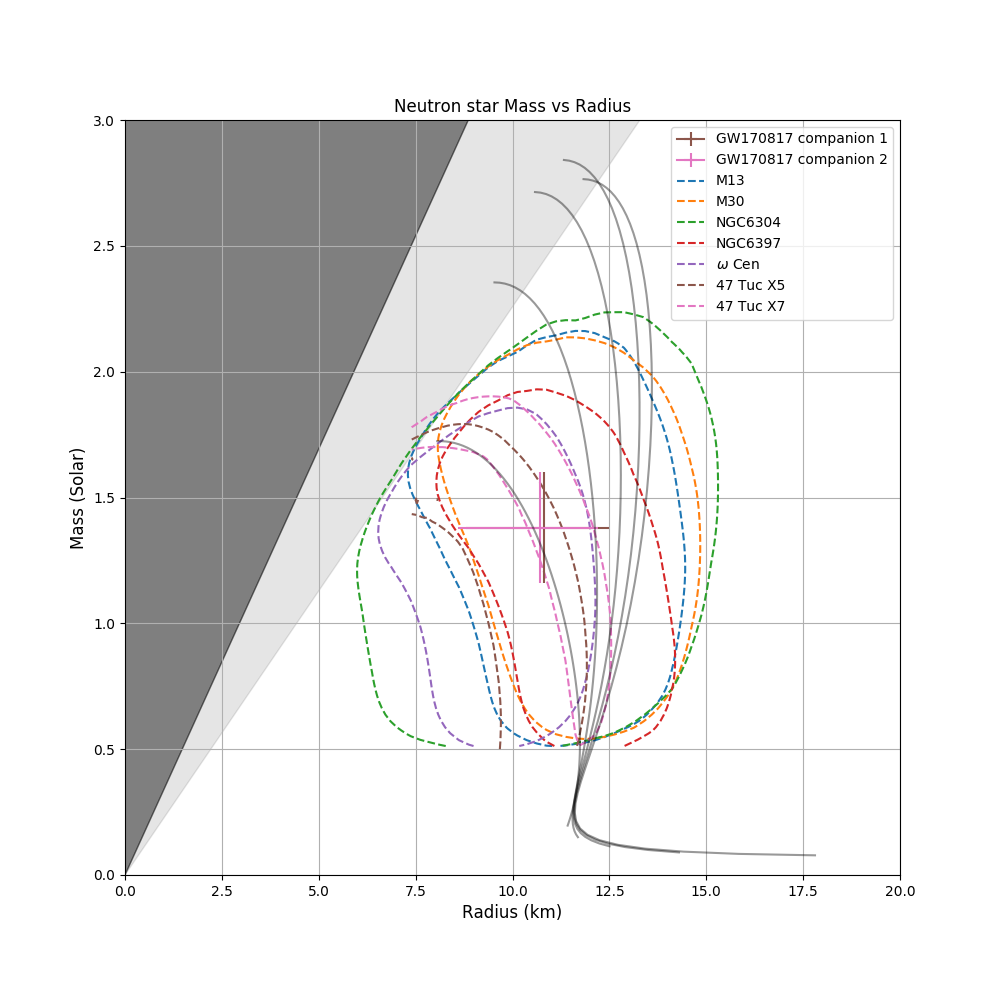
\includegraphics[width=\textwidth]{eos_compare_obsv2_GW}
                    \caption{Comparison between our model and the data from the LMXB thermonuclear burst and GW event}\label{fig/burst.LMXB}
                \end{subfigure}
                \caption{Comparison between our models and measured neutron star masses and radii}
            \end{center}\end{figure}
            
                We used two sources for the actual observed data of neutron stars: one is from the low mass X-ray binaries \parencite{ozel.psaltis.2016/radius.oberve} and the other is from the gravitational event caused by neutron star merge events \cite{ligo.virgo.2019/prop.of.ns.merger.GW170817,ligo.virgo.2018/GW170817.ns.radii}. The data from the LMXBs came in the form of likelihood as a function of a given mass-radius pair, which we plotted as contours of 68 percent confidence level. The Figure \ref{fig/quiescent.LMXB} shows the observational data from the quiescent LMXB, and Figure \ref{fig/burst.LMXB} shows the LMXB with thermonuclear bursts. On both figures we show the mass-radius relation of our model with different parameters for nuclear incompressibility and the calculated mass and radii of the neutron stars from the merger event GW170817. It can be seen from the both figure that the EOS with the parameters of $K_{0}=\SI{100}{\mega\electronvolt}$ and \SI{175}{\mega\electronvolt} falls within the 1 standard deviations of the LMXB observations while the EOS with other parameters do not due to having higher maximum masses. Comparing with the data from GW170817, EOSs with $K_{0}=\SI{175}{\mega\electronvolt}$ to \SI{400}{\mega\electronvolt} falls within 1 standard deviation and the EOS with $K_{0}=\SI{100}{\mega\electronvolt}$ within 2 standard deviations. Based on these facts we can estimate that the EOSs with the nuclear incompressibility $K_{0}=\SI{175}{\mega\electronvolt}$ and \SI{250}{\mega\electronvolt} are the most consistent with the observations.
        
        [Say the effect of nuclear interaction on the mass and radius]. [Compare the result with other models using diagram]. [Pick few models and explain a bit deeper, why they have their distinct shapes].
    
    \section{Conclusion}
        In this project we used 4th order Runge-Kutta method to numerically integrate the TOV structure equation to get the mass-radius relation of the neutron star. A neutron Fermi gas model and then a model with nucleon interactions of different strengths were considered. We found that the nucleon interactions has the effect of making the neutron star stiffer, thus increasing the maximum mass. For nuclear compressibilities of \SI{100}{\mega\electronvolt}, \SI{175}{\mega\electronvolt}, \SI{250}{\mega\electronvolt}, \SI{325}{\mega\electronvolt}, and \SI{400}{\mega\electronvolt} the maximum masses were determined to be \SI{1.36}{\solarmass}, \SI{2.01}{\solarmass}, \SI{2.30}{\solarmass}, \SI{2.27}{\solarmass}, and \SI{1.97}{\solarmass}, respectively. Upon comparing with the actual observed masses and radii of neutron stars in low mass X-ray binaries and of neutron star merger, the $K_0$ of \SI{175}{\mega\electronvolt} and \SI{250}{\mega\electronvolt} were found to be the most consistent with the data.
        
        The model used in this project is relatively simple: it dosn't consider the rotation of the star and it assumes there are only neutrons in the entire star. These can be adressed to make more realistic equation of states. Looking into the future, since the upgrade in the sensitivity of the LIGO detector in the spring of 2019, it is expected to detect gravitatonal wave event more frequently than in the previous years, so we can expect that there will be more precise data available on the masses  and radii of neutron stars that can further constrain the equation of state of the dense nuclear matter \cite{ligo.update.2019}.
    
    \printbibliography
\end{document}
